\documentclass[border=8pt]{standalone}
\usepackage[T1]{fontenc}
\usepackage[utf8]{inputenc}
\usepackage{mathptmx}          % Times, para coincidir con el cuerpo del informe
\usepackage{xcolor}
\usepackage{tikz}
\usetikzlibrary{positioning,arrows.meta,calc,fit,backgrounds,decorations.pathreplacing}

% Paleta
\definecolor{localFill}{HTML}{E8EEF6}
\definecolor{localDraw}{HTML}{2F5496}
\definecolor{remoteFill}{HTML}{FCEEDB}
\definecolor{remoteDraw}{HTML}{B5651D}
\definecolor{extFill}{HTML}{F0F0F0}
\definecolor{extDraw}{HTML}{7A7A7A}
\definecolor{arrowCol}{HTML}{3A3A3A}
\definecolor{zoneFill}{HTML}{FBF3E7}
\definecolor{zoneDraw}{HTML}{D9A86C}

\begin{document}
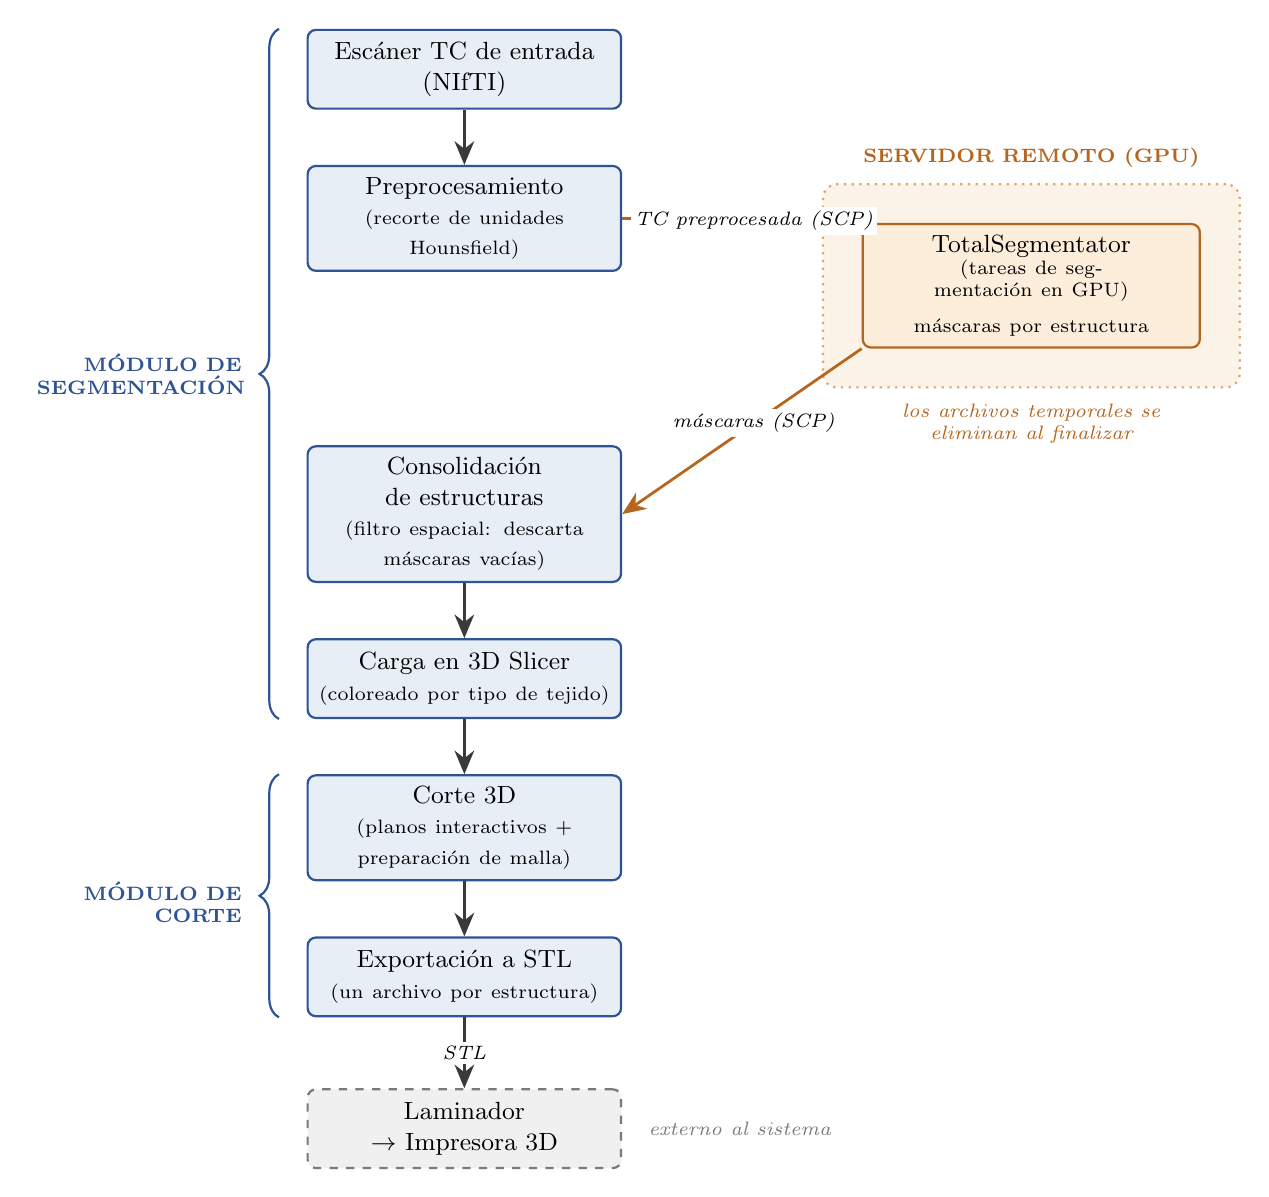
\begin{tikzpicture}[
  font=\small,
  box/.style={draw=localDraw, line width=0.8pt, rounded corners=3pt, fill=localFill,
              align=center, text width=3.7cm, minimum height=1.0cm, inner sep=4pt},
  remotebox/.style={draw=remoteDraw, line width=0.8pt, rounded corners=3pt, fill=remoteFill,
              align=center, text width=4.0cm, minimum height=1.1cm, inner sep=4pt},
  extbox/.style={draw=extDraw, line width=0.8pt, dashed, rounded corners=3pt, fill=extFill,
              align=center, text width=3.7cm, minimum height=1.0cm, inner sep=4pt},
  flow/.style={-{Stealth[length=3mm,width=2.5mm]}, line width=1.0pt, draw=arrowCol},
  scp/.style={-{Stealth[length=3mm,width=2.5mm]}, line width=1.0pt, draw=remoteDraw},
  lbl/.style={font=\scriptsize\itshape, fill=white, inner sep=1.5pt},
]

% ---- Columna local (vertical) ----
\node[box]                        (ct)    at (0,0) {Escáner TC de entrada\\(NIfTI)};
\node[box, below=0.7cm of ct]     (prep)           {Preprocesamiento\\\scriptsize(recorte de unidades Hounsfield)};
\node[box, below=2.2cm of prep]   (consol)         {Consolidación de estructuras\\\scriptsize(filtro espacial: descarta máscaras vacías)};
\node[box, below=0.7cm of consol] (slicer)         {Carga en 3D Slicer\\\scriptsize(coloreado por tipo de tejido)};
\node[box, below=0.7cm of slicer] (corte)          {Corte 3D\\\scriptsize(planos interactivos + preparación de malla)};
\node[box, below=0.7cm of corte]  (stl)            {Exportación a STL\\\scriptsize(un archivo por estructura)};
\node[extbox, below=0.9cm of stl] (lam)            {Laminador\\$\rightarrow$ Impresora 3D};

% ---- Servidor remoto (a la derecha) ----
\node[remotebox] (ts) at (7.2,-2.75) {TotalSegmentator\\\scriptsize(tareas de segmentación en GPU)\\[2pt]máscaras por estructura};

% ---- Flechas flujo vertical ----
\draw[flow] (ct)     -- (prep);
\draw[flow] (consol) -- (slicer);
\draw[flow] (slicer) -- (corte);
\draw[flow] (corte)  -- (stl);
\draw[flow] (stl)    -- (lam) node[lbl, midway] {STL};

% ---- Flechas SCP (ida y vuelta al servidor), con anclas separadas ----
\draw[scp] (prep.east)   -- (ts.north west) node[lbl, pos=0.55] {TC preprocesada (SCP)};
\draw[scp] (ts.south west) -- (consol.east) node[lbl, pos=0.45] {máscaras (SCP)};

% ---- Zona remota (fondo) ----
\begin{scope}[on background layer]
  \node[draw=zoneDraw, line width=0.8pt, dotted, rounded corners=5pt, fill=zoneFill,
        fit=(ts), inner sep=14pt] (zona) {};
\end{scope}
\node[font=\scriptsize\bfseries, text=remoteDraw, anchor=south]
      at ([yshift=2pt]zona.north) {SERVIDOR REMOTO (GPU)};
\node[font=\scriptsize\itshape, text=remoteDraw, anchor=north, align=center]
      at ([yshift=-2pt]zona.south) {los archivos temporales se\\eliminan al finalizar};

% ---- Brackets de módulos (izquierda) ----
\draw[decorate, decoration={brace, amplitude=7pt}, line width=0.8pt, draw=localDraw]
  ($(slicer.south west)+(-0.35,0)$) -- ($(ct.north west)+(-0.35,0)$);
\node[text=localDraw, font=\scriptsize\bfseries, text width=2.6cm, align=right, anchor=east]
  at ($(ct.west)!0.5!(slicer.west)+(-0.7,0)$) {MÓDULO DE\\SEGMENTACIÓN};

\draw[decorate, decoration={brace, amplitude=7pt}, line width=0.8pt, draw=localDraw]
  ($(stl.south west)+(-0.35,0)$) -- ($(corte.north west)+(-0.35,0)$);
\node[text=localDraw, font=\scriptsize\bfseries, text width=2.6cm, align=right, anchor=east]
  at ($(corte.west)!0.5!(stl.west)+(-0.7,0)$) {MÓDULO DE\\CORTE};

% ---- Etiqueta "externo" ----
\node[font=\scriptsize\itshape, text=extDraw, anchor=west] at ([xshift=6pt]lam.east) {externo al sistema};

\end{tikzpicture}
\end{document}